\subsection{Model Dynamics}
\label{sec:og.dynamics}
\label{sec:state.og.dynamics}

We are interested in the dynamics that emerge when fixing the parameters $\beta = 1, f = 150, L = 4.2 \cdot 10^{-3}, R = 2, V_m = 5,$ and $\mu = 0.5$.
The parameters $E_0$ and $\chi_0$ are varied.
$E_0$ is in the range $[14, 28]$, while $\chi_0$ is in the range $[0.1, 0.65]$.
Scanning this parameter plane for the period of stable cycles results in \Cref{fig:yunus.2pi.2d.full}.

\begin{figure}
	\centering
	\includegraphics[width=0.6\textwidth]{99_Yunus/2D_Period_Zoomed/result.png}
	\caption{2D Scan of Original Model}
	\label{fig:yunus.2pi.2d.full}
\end{figure}

The regions in \Cref{fig:yunus.2pi.2d.full} with the same color mean, that the stable cycles in these regions have the same period.
Points $A, B$ and $C$ are in the parameter region, which has stable cycles with the period 12.
The period regions, in which these points are, differ in another way.
Besides the period of a cycle, there is another characteristic, the symbolic sequence.
As mentioned before, it describes on which branches of the model function the points of the cycle exist.
Some cobwebs illustrate the difference between the parameter regions.
\Cref{fig:yunus.2pi.CobwebA12,fig:yunus.2pi.CobwebC12} show the cobwebs at points $A$ and $C$.
Both parameter regions have only one stable cycle of period 12.
The stable cycle at point $A$ has the symbolic sequence $\A^3\B^3\C^3\D^3$ and the cycle at point $C$ has the symbolic sequence $\A^2\B^4\C^2\D^4$.
We follow the convention, that the branch with the smallest positive boundaries is called branch $\A$.
We say that such parameter regions are of ``type A'', while the parameter region for point $B$ is of ``type B''.

\Cref{fig:yunus.2pi.CobwebB12} shows the cobweb at point $B$.
We see directly that there are now two coexisting cycles of period 12.
One cycle has the symbolic sequence $\A^3\B^3\C^2\D^4$, while the other one has the symbolic sequence $\A^2\B^2\C^3\D^3$
We say that both of these are symmetric by rotating the cycle by $\pi$, meaning the two halves of the cycles are swapped.
These cycles behave similarly to both the cycles at points $A$ and $B$ in the following way.
The cycle $\Cycle{\A^3\B^3\C^2\D^4}$ behaves like the cycle $\Cycle{\A^3\B^3\C^3\D^3}$ at point $A$ on its left half, while it behaves like the cycle $\Cycle{\A^2\B^4\C^2\D^4}$ on its right half.
The same is true for the cycle $\Cycle{\A^2\B^4\C^3\D^3}$ but reversed since it is the other cycle rotated by $\pi$.

\begin{figure}
	\centering
	\begin{subfigure}{0.3\textwidth}
		\centering
		\includegraphics[width=\textwidth]{99_Yunus/Period12/Cobweb_A_12/result.png}
		\caption{At Point $A$}
		\label{fig:yunus.2pi.CobwebA12}
	\end{subfigure}
	\begin{subfigure}{0.3\textwidth}
		\centering
		\includegraphics[width=\textwidth]{99_Yunus/Period12/Cobweb_B_12/result.png}
		\caption{At Point $B$}
		\label{fig:yunus.2pi.CobwebB12}
	\end{subfigure}
	\begin{subfigure}{0.3\textwidth}
		\centering
		\includegraphics[width=\textwidth]{99_Yunus/Period12/Cobweb_C_12/result.png}
		\caption{At Point $C$}
		\label{fig:yunus.2pi.CobwebC12}
	\end{subfigure}
	\caption{Cobwebs of Full Original Model}
\end{figure}

This behavior is peculiar.
To summarize, we have chains of parameter regions with the same period.
The type of the parameter regions alternates between ``type A'' and ``type B''.
When the stable cycle in one ``type A'' parameter region is $\A^x\B^y\C^x\D^y$, the stable cycle in the next ``type A'' parameter region is $\A^{x-1}\B^{y+1}\C^{x-1}\D^{y+1}$.
The ``type B'' parameter region in between two ``type A'' parameter regions of a chain with cycles $\A^x\B^y\C^x\D^y$ and $\A^{x-1}\B^{y+1}\C^{x-1}\D^{y+1}$, has the two cycles $\A^x\B^y\C^{x-1}\D^{y+1}$ and $\A^{x-1}\B^{y+1}\C^x\D^y$.
Also, there is not only one chain, but many chains next to each other where the period increases by 2 from one chain to the next.

\begin{align}
	F(\theta + \pi) & \equiv F(\theta) + \pi \mod 2 \pi \label{equ:state.og.sym}
\end{align}

The model has some symmetry, it satisfies \Cref{equ:state.og.sym}.
This means, that the model behaves the same on the left half as it does on the right half.
In ``type A'' parameter regions, the stable cycles are symmetric.
But in ``type B'' parameter regions, the stable cycles are asymmetric.
